\documentclass[aspectratio=169,fleqn]{beamer}
\usepackage{spc}
\usepackage{graphicx}
\begin{document}

\begin{frame}
  \title{\vspace{-5ex}\darkblue Scoping the next stock assessment
    platform\\[2ex]
    \it\large\darkgray
    Stage I: Reaching out to tuna RFMOs and the scientific community}
  \author{\vspace{-10ex}\darkgray\bf
    Arni Magnusson, Nick Davies}
  \date{\darkgreen SPC international expert meeting (online)\\[0.5ex]
    13 May and 18 June 2024}
  \titlepage
\end{frame}

% ______________________________________________________________________________

\begin{frame}{Meeting Objectives}
  \begin{itemize}
    \item[] {\bf\darkblue Communicate} \comment{project 123, explorations,
      decisions, development}\\[5ex]
    \item[] {\bf\darkblue Discuss} \comment{succession plans, admb, multifan-cl,
      stock synthesis}\\[5ex]
    \item[] {\bf\darkblue Seek Advice} \comment{insights, opinions, experiences,
      predictions, ideas}\\[5ex]
    \item[] {\bf\darkblue Seek Collaboration} \comment{tuna RFMOs, research
      labs}\\[1ex]
  \end{itemize}
\end{frame}

% ______________________________________________________________________________

\begin{frame}{Meeting Schedule}\small
  \begin{tabular}{ll}
    $\Rightarrow$ \gray 0:00\h{0.3ex}--\h{0.3ex}0:20
    & Introduction\\[1.6ex]
    \h{3ex}\gray 0:20\h{0.3ex}--\h{0.3ex}0:30
    & {\bf Platforms} currently used in tuna stock assessments
      {\gray (presentation, round table)}\\[1.6ex]
    \h{3ex}\gray 0:30\h{0.3ex}--\h{0.3ex}0:50
    & {\bf\green Common challenges} for all tuna RFMOs, {\bf\green longevity} of
      Stock Synthesis\\[0.6ex]
    ~ & and MULTIFAN-CL, {\bf\green succession plans} {\gray (round
        table)}\\[1.6ex]
    \h{3ex}\gray 0:50\h{0.3ex}--\h{0.3ex}1:00
    & SPC challenges and {\bf project plan} {\gray (presentation)}\\[1.6ex]
    \h{3ex}\gray 1:00\h{0.3ex}--\h{0.3ex}1:10
    & {\bf Features} of current and future platforms {\gray
      (presentation)}\\[1.6ex]
    \h{3ex}\gray 1:10\h{0.3ex}--\h{0.3ex}1:25
    & Discussion on platform {\bf\green features} most {\bf\green relevant for
      tuna} {\gray (round table)}\\[1.6ex]
    \h{3ex}\gray 1:25\h{0.3ex}--\h{0.3ex}1:35
    & {\bf State-space} models and latest developments {\gray
      (presentation)}\\[1.6ex]
    \h{3ex}\gray 1:35\h{0.3ex}--\h{0.3ex}1:50
    & What do you think is the {\bf\green best way forward for SPC?} {\gray
      (round table)}\\[1.6ex]
    \h{3ex}\gray 1:50\h{0.3ex}--\h{0.3ex}2:00
    & Summary of discussions, next steps, {\bf\green collaboration} {\gray
      (round table)}\\[1.6ex]
  \end{tabular}
\end{frame}

% ______________________________________________________________________________

\begin{frame}{Who Are Here Today?}
  People with expertise in\\[1.5ex]
  \begin{itemize}
    \item Tuna\\[2ex]
    \item Stock assessment\\[2ex]
    \item Software development\\[2ex]
  \end{itemize}
  \qquad\green ---\\[2ex]
  \quad\comment{What is your main line of work?}\\[2ex]
  \quad\comment{What part of your work is related to tuna/stock
    assessment/software development?}
\end{frame}

% ______________________________________________________________________________

\begin{frame}{~}\small
  \begin{tabular}{ll}
    \h{3ex}\gray 0:00\h{0.3ex}--\h{0.3ex}0:20
    & Introduction\\[1.6ex]
    $\Rightarrow$ \gray 0:20\h{0.3ex}--\h{0.3ex}0:30
    & {\bf Platforms} currently used in tuna stock assessments
      {\gray (presentation, round table)}\\[1.6ex]
    \h{3ex}\gray 0:30\h{0.3ex}--\h{0.3ex}0:50
    & {\bf\green Common challenges} for all tuna RFMOs, {\bf\green longevity} of
      Stock Synthesis\\[0.6ex]
    ~ & and MULTIFAN-CL, {\bf\green succession plans} {\gray (round
        table)}\\[1.6ex]
    \h{3ex}\gray 0:50\h{0.3ex}--\h{0.3ex}1:00
    & SPC challenges and {\bf project plan} {\gray (presentation)}\\[1.6ex]
    \h{3ex}\gray 1:00\h{0.3ex}--\h{0.3ex}1:10
    & {\bf Features} of current and future platforms {\gray
      (presentation)}\\[1.6ex]
    \h{3ex}\gray 1:10\h{0.3ex}--\h{0.3ex}1:25
    & Discussion on platform {\bf\green features} most {\bf\green relevant for
      tuna} {\gray (round table)}\\[1.6ex]
    \h{3ex}\gray 1:25\h{0.3ex}--\h{0.3ex}1:35
    & {\bf State-space} models and latest developments {\gray
      (presentation)}\\[1.6ex]
    \h{3ex}\gray 1:35\h{0.3ex}--\h{0.3ex}1:50
    & What do you think is the {\bf\green best way forward for SPC?} {\gray
      (round table)}\\[1.6ex]
    \h{3ex}\gray 1:50\h{0.3ex}--\h{0.3ex}2:00
    & Summary of discussions, next steps, {\bf\green collaboration} {\gray
      (round table)}\\[1.6ex]
  \end{tabular}
\end{frame}

% ______________________________________________________________________________

\begin{frame}{Platforms currently used in tuna stock assessments}\small
  \begin{tabular}{lll}
    ICCAT & Atlantic & {\bf\blue Stock Synthesis}, JABBA, one-off models\\[3ex]
    IOTC & Indian & {\bf\blue Stock Synthesis} for all stocks?\\[3ex]
    IATTC & Pacific, Eastern & {\bf\blue Stock Synthesis} for all stocks?\\[3ex]
    SPC & Pacific, Western \& Central
                     & {\bf\green MULTIFAN-CL} for all stocks\\[3ex]
    CCSBT & Southern bluefin tuna & {\bf\orange sbt}, designed around CKMR\\
  \end{tabular}
\end{frame}

% ______________________________________________________________________________

\begin{frame}{~}\small
  \begin{tabular}{ll}
    \h{3ex}\gray 0:00\h{0.3ex}--\h{0.3ex}0:20
    & Introduction\\[1.6ex]
    \h{3ex}\gray 0:20\h{0.3ex}--\h{0.3ex}0:30
    & {\bf Platforms} currently used in tuna stock assessments
      {\gray (presentation, round table)}\\[1.6ex]
    $\Rightarrow$ \gray 0:30\h{0.3ex}--\h{0.3ex}0:50
    & {\bf\green Common challenges} for all tuna RFMOs, {\bf\green longevity} of
      Stock Synthesis\\[0.6ex]
    ~ & and MULTIFAN-CL, {\bf\green succession plans} {\gray (round
        table)}\\[1.6ex]
    \h{3ex}\gray 0:50\h{0.3ex}--\h{0.3ex}1:00
    & SPC challenges and {\bf project plan} {\gray (presentation)}\\[1.6ex]
    \h{3ex}\gray 1:00\h{0.3ex}--\h{0.3ex}1:10
    & {\bf Features} of current and future platforms {\gray
      (presentation)}\\[1.6ex]
    \h{3ex}\gray 1:10\h{0.3ex}--\h{0.3ex}1:25
    & Discussion on platform {\bf\green features} most {\bf\green relevant for
      tuna} {\gray (round table)}\\[1.6ex]
    \h{3ex}\gray 1:25\h{0.3ex}--\h{0.3ex}1:35
    & {\bf State-space} models and latest developments {\gray
      (presentation)}\\[1.6ex]
    \h{3ex}\gray 1:35\h{0.3ex}--\h{0.3ex}1:50
    & What do you think is the {\bf\green best way forward for SPC?} {\gray
      (round table)}\\[1.6ex]
    \h{3ex}\gray 1:50\h{0.3ex}--\h{0.3ex}2:00
    & Summary of discussions, next steps, {\bf\green collaboration} {\gray
      (round table)}\\[1.6ex]
  \end{tabular}
\end{frame}

% ______________________________________________________________________________

\begin{frame}{Round Table}
  \begin{itemize}
    \item Common challenges for all tuna RFMOs\\[5ex]
    \item Longevity of Stock Synthesis and MULTIFAN-CL\\[5ex]
    \item Succession plans\\[3ex]
  \end{itemize}
\end{frame}

% ______________________________________________________________________________

\begin{frame}{~}\small
  \begin{tabular}{ll}
    \h{3ex}\gray 0:00\h{0.3ex}--\h{0.3ex}0:20
    & Introduction\\[1.6ex]
    \h{3ex}\gray 0:20\h{0.3ex}--\h{0.3ex}0:30
    & {\bf Platforms} currently used in tuna stock assessments
      {\gray (presentation, round table)}\\[1.6ex]
    \h{3ex}\gray 0:30\h{0.3ex}--\h{0.3ex}0:50
    & {\bf\green Common challenges} for all tuna RFMOs, {\bf\green longevity} of
      Stock Synthesis\\[0.6ex]
    ~ & and MULTIFAN-CL, {\bf\green succession plans} {\gray (round
        table)}\\[1.6ex]
    $\Rightarrow$ \gray 0:50\h{0.3ex}--\h{0.3ex}1:00
    & SPC challenges and {\bf project plan} {\gray (presentation)}\\[1.6ex]
    \h{3ex}\gray 1:00\h{0.3ex}--\h{0.3ex}1:10
    & {\bf Features} of current and future platforms {\gray
      (presentation)}\\[1.6ex]
    \h{3ex}\gray 1:10\h{0.3ex}--\h{0.3ex}1:25
    & Discussion on platform {\bf\green features} most {\bf\green relevant for
      tuna} {\gray (round table)}\\[1.6ex]
    \h{3ex}\gray 1:25\h{0.3ex}--\h{0.3ex}1:35
    & {\bf State-space} models and latest developments {\gray
      (presentation)}\\[1.6ex]
    \h{3ex}\gray 1:35\h{0.3ex}--\h{0.3ex}1:50
    & What do you think is the {\bf\green best way forward for SPC?} {\gray
      (round table)}\\[1.6ex]
    \h{3ex}\gray 1:50\h{0.3ex}--\h{0.3ex}2:00
    & Summary of discussions, next steps, {\bf\green collaboration} {\gray
      (round table)}\\[1.6ex]
  \end{tabular}
\end{frame}

% ______________________________________________________________________________

\begin{frame}{SPC Challenges}\small
  \begin{itemize}
    \item[] MFCL Team (Dave Fournier, John Hampton, Nick Davies) retiring in the
    2020s\\[5ex]
    \item[] Quick turnover rate of stock assessment staff\\[5ex]
    \item[] Takes many years to become an expert in MFCL, John typically makes
    the main\\[0.2ex]
    modeling decisions and guides new staff, with the help of Nick\\[5ex]
    \item[] We must prepare for an era where there might be no long-term staff,
    only short-term\\[3ex]
  \end{itemize}
\end{frame}

% ______________________________________________________________________________

\begin{frame}{Project P123}\small
  \begin{itemize}
    \item[] Scoping the next tuna stock assessment software\\[3ex]
    \item[] Project scheduled 1 Feb 2024 to 31 Dec 2026\\[3ex]
    \item[] This initial project will:
    \begin{itemize}
      \item[-] evaluate {\green features and capabilities} that will be
      important in future tuna assessments\\[1ex]
      \item[-] explore fitting models to tuna data using {\green existing
        software platforms}\\[1ex]
      \item[-] guide decisions on what kind of {\green new software development}
      will be required\\[1ex]
      \item[-] establish {\green collaboration} with tRFMOs and research labs to
      achieve these goals\\[3ex]
    \end{itemize}
    Additional projects can be launched in parallel to power up the model
    exploration and software development
  \end{itemize}
\end{frame}

% ______________________________________________________________________________

\begin{frame}{Project Plan}\small
  \textit{2024}
  \begin{itemize}
    \item[1.] Review and identify important model features for tuna
    assessments\\[-1ex]
    \item[2.] Identify existing platforms that have these features or can be
    extended\\[-1ex]
    \item[3.] Reach out to and initiate collaboration with model
    developers\\[-1ex]
    \item[4.] Conduct two workshops in 2024, one online and one in person\\[4ex]
  \end{itemize}
  \textit{2025\h{0.2ex}--\h{0.2ex}2026}
  \begin{itemize}
    \item[5.] Explore and compare existing platforms, fitting to SPC tuna
    data\\[-1ex]
    \item[6.] Determine which platforms can be considered viable
    candidates\\[-1ex]
    \item[7.] If a viable platform has been identified, plan transition\\[-1ex]
    \item[8.] If no viable platform is identified, launch a software
    development\\[0.1ex]
    project to extend a platform or create a new one
  \end{itemize}
\end{frame}

% ______________________________________________________________________________

\begin{frame}[plain]
  \begin{tikzpicture}[remember picture,overlay]
    \node[at=(current page.center)]%
    {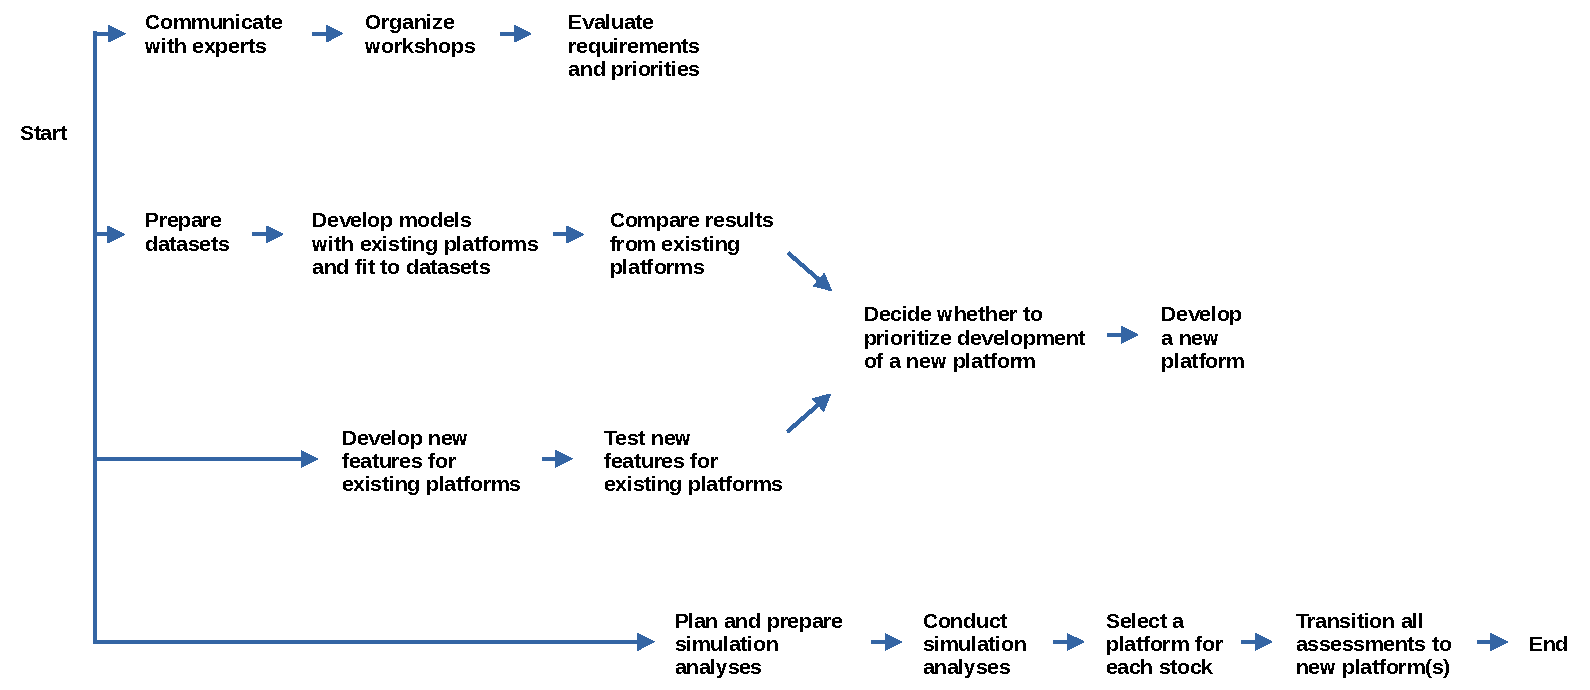
\includegraphics[width=0.95\paperwidth]{p123_diagram}};
  \end{tikzpicture}
\end{frame}

% ______________________________________________________________________________

\begin{frame}{~}\small
  \begin{tabular}{ll}
    \h{3ex}\gray 0:00\h{0.3ex}--\h{0.3ex}0:20
    & Introduction\\[1.6ex]
    \h{3ex}\gray 0:20\h{0.3ex}--\h{0.3ex}0:30
    & {\bf Platforms} currently used in tuna stock assessments
      {\gray (presentation, round table)}\\[1.6ex]
    \h{3ex}\gray 0:30\h{0.3ex}--\h{0.3ex}0:50
    & {\bf\green Common challenges} for all tuna RFMOs, {\bf\green longevity} of
      Stock Synthesis\\[0.6ex]
    ~ & and MULTIFAN-CL, {\bf\green succession plans} {\gray (round
        table)}\\[1.6ex]
    \h{3ex}\gray 0:50\h{0.3ex}--\h{0.3ex}1:00
    & SPC challenges and {\bf project plan} {\gray (presentation)}\\[1.6ex]
    $\Rightarrow$ \gray 1:00\h{0.3ex}--\h{0.3ex}1:10
    & {\bf Features} of current and future platforms {\gray
      (presentation)}\\[1.6ex]
    \h{3ex}\gray 1:10\h{0.3ex}--\h{0.3ex}1:25
    & Discussion on platform {\bf\green features} most {\bf\green relevant for
      tuna} {\gray (round table)}\\[1.6ex]
    \h{3ex}\gray 1:25\h{0.3ex}--\h{0.3ex}1:35
    & {\bf State-space} models and latest developments {\gray
      (presentation)}\\[1.6ex]
    \h{3ex}\gray 1:35\h{0.3ex}--\h{0.3ex}1:50
    & What do you think is the {\bf\green best way forward for SPC?} {\gray
      (round table)}\\[1.6ex]
    \h{3ex}\gray 1:50\h{0.3ex}--\h{0.3ex}2:00
    & Summary of discussions, next steps, {\bf\green collaboration} {\gray
      (round table)}\\[1.6ex]
  \end{tabular}
\end{frame}

% ______________________________________________________________________________

\begin{frame}{Tuna Models, Regions and Tags}\small\href%
  {https://github.com/PacificCommunity/ofp-sam-transition-plan/blob/main/presentations/2024_05_13_mfcl_future/MULTIFAN-CL_future.pdf}%
  {\blue Presentation} by Nick Davies, SPC
\end{frame}

% ______________________________________________________________________________

\begin{frame}{Features of Current Platforms (CAPAM 2019)}\fns
  ~\hspace{-4ex}%
  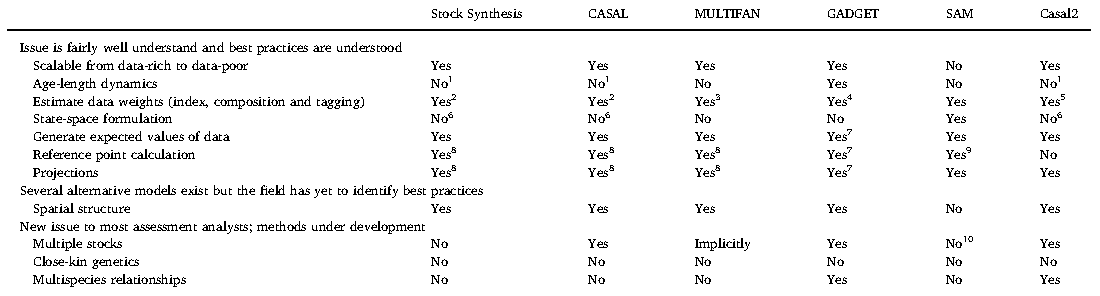
\includegraphics[width=1.08\textwidth]{capam_2019_paper_features}\\[1ex]
  \gray\scriptsize (CAPAM 2019 paper)
\end{frame}

% ______________________________________________________________________________

\begin{frame}{Structural Features of Current Platforms}\fns
  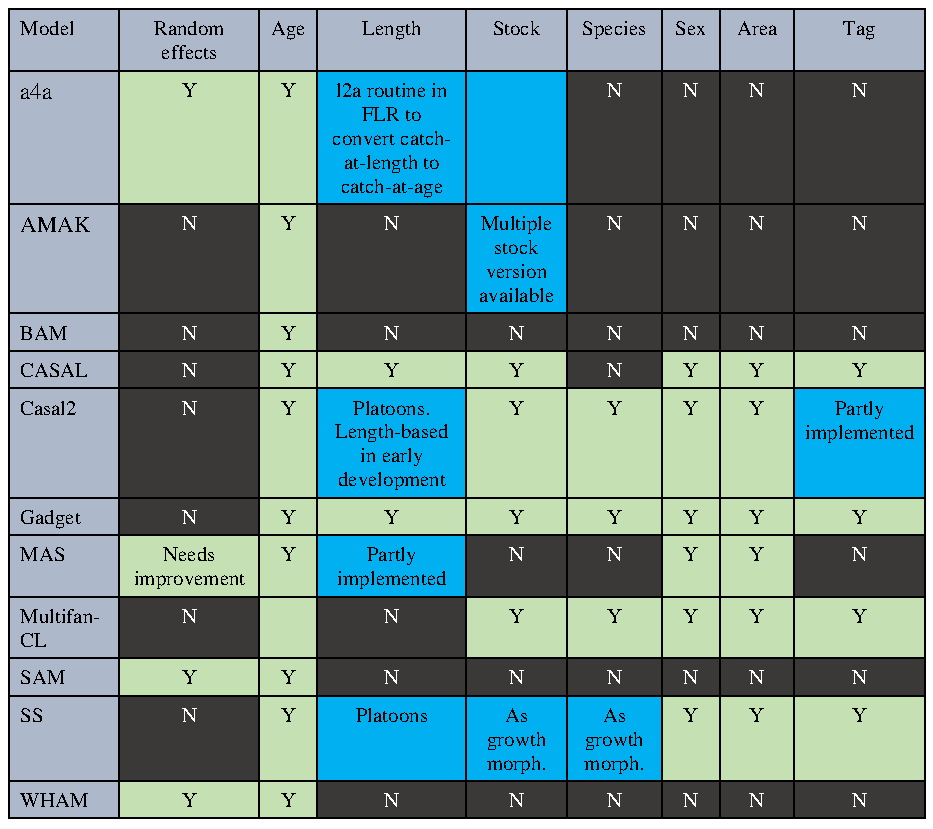
\includegraphics[width=0.85\textwidth]{capam_2019_report_features}\\[2ex]
  \gray\scriptsize (CAPAM 2019 report)
\end{frame}

% ______________________________________________________________________________

\begin{frame}{Modifications Needed}\fns
  \vspace{4ex}
  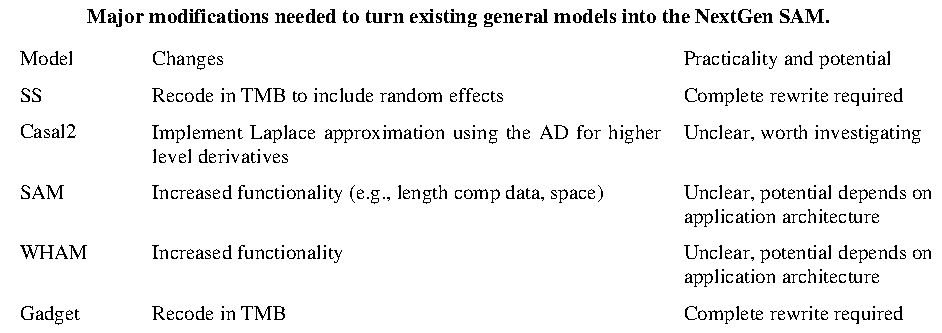
\includegraphics[width=0.95\textwidth]{capam_2019_report_development}\\[5ex]
  \gray\scriptsize (CAPAM 2019 report)
\end{frame}

% ______________________________________________________________________________

\begin{frame}{Features of Current and Future Platforms}\small
  \vspace{-1.5ex}
  \begin{columns}[T]
    \column{0.5\textwidth}\gray
    Incorporating data\\[-0.5ex]
    \begin{itemize}\fns
      \item Fit to length comps\\[-1ex]
      \item Fit to weight comps\\[-1ex]
      \item Fit to tagging data\\[-1ex]
      \item Fit to CKMR data\\[-1ex]
      \item Estimate growth curve using otolith data\\[-1ex]
      \item Utilize tag-recapture growth increment to estimate growth\\[3ex]
    \end{itemize}
    Specifics\\[-0.5ex]
    \begin{itemize}\fns
      \item Age-specific M\\[-1ex]
      \item Length-specific selectivity\\[-1ex]
      \item Sex-specific growth and M\\[-1ex]
      \item Region-specific growth\\[3ex]
    \end{itemize}
    \column{0.5\textwidth}\gray
    Dimensions\\[-0.5ex]
    \begin{itemize}\fns
      \item Explicit regions with movement\\[-1ex]
      \item Tracking age and length in population\\[-1ex]
      \item Time steps within a year\\[3ex]
    \end{itemize}
    Ecology\\[-0.5ex]
    \begin{itemize}\fns
      \item Multispecies interactions\\[-1ex]
      \item Climate change\\[3ex]
    \end{itemize}
    Implementation\\[-0.5ex]
    \begin{itemize}\fns
      \item Random effects, state space\\[-1ex]
      \item Parallel computing\\[-1ex]
      \item Computation time
    \end{itemize}
  \end{columns}
\end{frame}

% ______________________________________________________________________________

\begin{frame}{~}\small
  \begin{tabular}{ll}
    \h{3ex}\gray 0:00\h{0.3ex}--\h{0.3ex}0:20
    & Introduction\\[1.6ex]
    \h{3ex}\gray 0:20\h{0.3ex}--\h{0.3ex}0:30
    & {\bf Platforms} currently used in tuna stock assessments
      {\gray (presentation, round table)}\\[1.6ex]
    \h{3ex}\gray 0:30\h{0.3ex}--\h{0.3ex}0:50
    & {\bf\green Common challenges} for all tuna RFMOs, {\bf\green longevity} of
      Stock Synthesis\\[0.6ex]
    ~ & and MULTIFAN-CL, {\bf\green succession plans} {\gray (round
        table)}\\[1.6ex]
    \h{3ex}\gray 0:50\h{0.3ex}--\h{0.3ex}1:00
    & SPC challenges and {\bf project plan} {\gray (presentation)}\\[1.6ex]
    \h{3ex}\gray 1:00\h{0.3ex}--\h{0.3ex}1:10
    & {\bf Features} of current and future platforms {\gray
      (presentation)}\\[1.6ex]
    $\Rightarrow$ \gray 1:10\h{0.3ex}--\h{0.3ex}1:25
    & Discussion on platform {\bf\green features} most {\bf\green relevant for
      tuna} {\gray (round table)}\\[1.6ex]
    \h{3ex}\gray 1:25\h{0.3ex}--\h{0.3ex}1:35
    & {\bf State-space} models and latest developments {\gray
      (presentation)}\\[1.6ex]
    \h{3ex}\gray 1:35\h{0.3ex}--\h{0.3ex}1:50
    & What do you think is the {\bf\green best way forward for SPC?} {\gray
      (round table)}\\[1.6ex]
    \h{3ex}\gray 1:50\h{0.3ex}--\h{0.3ex}2:00
    & Summary of discussions, next steps, {\bf\green collaboration} {\gray
      (round table)}\\[1.6ex]
  \end{tabular}
\end{frame}

% ______________________________________________________________________________

\begin{frame}{~}\small
  \begin{tabular}{ll}
    \h{3ex}\gray 0:00\h{0.3ex}--\h{0.3ex}0:20
    & Introduction\\[1.6ex]
    \h{3ex}\gray 0:20\h{0.3ex}--\h{0.3ex}0:30
    & {\bf Platforms} currently used in tuna stock assessments
      {\gray (presentation, round table)}\\[1.6ex]
    \h{3ex}\gray 0:30\h{0.3ex}--\h{0.3ex}0:50
    & {\bf\green Common challenges} for all tuna RFMOs, {\bf\green longevity} of
      Stock Synthesis\\[0.6ex]
    ~ & and MULTIFAN-CL, {\bf\green succession plans} {\gray (round
        table)}\\[1.6ex]
    \h{3ex}\gray 0:50\h{0.3ex}--\h{0.3ex}1:00
    & SPC challenges and {\bf project plan} {\gray (presentation)}\\[1.6ex]
    \h{3ex}\gray 1:00\h{0.3ex}--\h{0.3ex}1:10
    & {\bf Features} of current and future platforms {\gray
      (presentation)}\\[1.6ex]
    \h{3ex}\gray 1:10\h{0.3ex}--\h{0.3ex}1:25
    & Discussion on platform {\bf\green features} most {\bf\green relevant for
      tuna} {\gray (round table)}\\[1.6ex]
    $\Rightarrow$ \gray 1:25\h{0.3ex}--\h{0.3ex}1:35
    & {\bf State-space} models and latest developments {\gray
      (presentation)}\\[1.6ex]
    \h{3ex}\gray 1:35\h{0.3ex}--\h{0.3ex}1:50
    & What do you think is the {\bf\green best way forward for SPC?} {\gray
      (round table)}\\[1.6ex]
    \h{3ex}\gray 1:50\h{0.3ex}--\h{0.3ex}2:00
    & Summary of discussions, next steps, {\bf\green collaboration} {\gray
      (round table)}\\[1.6ex]
  \end{tabular}
\end{frame}

% ______________________________________________________________________________

\begin{frame}{State-Space Models}\normalsize
  {\green Deterministic}
  \begin{displaymath}
    N_{t+1,a+1} \;\;=\;\; N_{t,a} \;\times\; e^{-(F_{t,a}\,+\,M_{t,a})}
  \end{displaymath}
  ~\\[2ex]
  {\orange State-space}
  \begin{displaymath}
    N_{t+1,a+1} \;\;=\;\; N_{t,a} \;\times\;
    e^{-(F_{t,a}\,+\,M_{t,a}\,+\,\eta_{t,a})}
  \end{displaymath}
\end{frame}

% ______________________________________________________________________________

\begin{frame}{Recent and Ongoing Development}\small
  \begin{tabular}{lll}
    ALSCL & state-space tracking age-length
    & \comment{\fns Fan Zhang, Noel Cadigan}\\[1.5ex]
    FIMS & age-structured case studies & \comment{\fns NOAA}\\[1.5ex]
    Gadget3 & ported to TMB, has CKMR
    & \comment{\fns Jamie Lentin, Bjarki Elvarsson, Will Butler}\\[1.5ex]
    sbt & ported to TMB, has CKMR
    & \comment{\fns D'Arcy Webber, Rich Hillary}\\[1.5ex]
    SS+ckmr & CKMR module for SS & \comment{\fns André Punt, CSIRO}\\[1.5ex]
    SS+tag & enhanced tag module for SS
    & \comment{\fns Nicholas Ducharme-Barth, Arni Magnusson}\\[1.5ex]
    SAM+length & fitted to length comps
    & \comment{\fns Colin Millar, Anders Nielsen}\\[1.5ex]
    WHAM+length & fitted to length comps
    & \comment{\fns Giancarlo Correa, Tim Miller}\\[1.5ex]
  \end{tabular}
\end{frame}

% ______________________________________________________________________________

\begin{frame}{Pathways to a State-Space Model for Tuna Assessments}\small
  \begin{tabular}{ll}
    \hline
    \bf Starting point & \bf Add features\I{2.5ex}\\[0.2ex]
    \hline
    ALSCL          & catch data, tags, regions, CKMR\I{2.5ex}\\[0.5ex]
    Casal2         & state space, CKMR\\[0.5ex]
    FIMS           & state space, fit to length comps, regions, CKMR\\[0.5ex]
    Gadget3        & state space\\[0.5ex]
    sbt            & regions\\[0.5ex]
    SS             & state space, tags, CKMR\\[0.5ex]
    SAM            & fit to length comps, regions, CKMR\\[0.5ex]
    WHAM           & fit to length comps, regions, CKMR\\[0.2ex]
    \hline
  \end{tabular}
  \vspace{4ex}
\end{frame}

% ______________________________________________________________________________

\begin{frame}{~}\small
  \begin{tabular}{ll}
    \h{3ex}\gray 0:00\h{0.3ex}--\h{0.3ex}0:20
    & Introduction\\[1.6ex]
    \h{3ex}\gray 0:20\h{0.3ex}--\h{0.3ex}0:30
    & {\bf Platforms} currently used in tuna stock assessments
      {\gray (presentation, round table)}\\[1.6ex]
    \h{3ex}\gray 0:30\h{0.3ex}--\h{0.3ex}0:50
    & {\bf\green Common challenges} for all tuna RFMOs, {\bf\green longevity} of
      Stock Synthesis\\[0.6ex]
    ~ & and MULTIFAN-CL, {\bf\green succession plans} {\gray (round
        table)}\\[1.6ex]
    \h{3ex}\gray 0:50\h{0.3ex}--\h{0.3ex}1:00
    & SPC challenges and {\bf project plan} {\gray (presentation)}\\[1.6ex]
    \h{3ex}\gray 1:00\h{0.3ex}--\h{0.3ex}1:10
    & {\bf Features} of current and future platforms {\gray
      (presentation)}\\[1.6ex]
    \h{3ex}\gray 1:10\h{0.3ex}--\h{0.3ex}1:25
    & Discussion on platform {\bf\green features} most {\bf\green relevant for
      tuna} {\gray (round table)}\\[1.6ex]
    \h{3ex}\gray 1:25\h{0.3ex}--\h{0.3ex}1:35
    & {\bf State-space} models and latest developments {\gray
      (presentation)}\\[1.6ex]
    $\Rightarrow$ \gray 1:35\h{0.3ex}--\h{0.3ex}1:50
    & What do you think is the {\bf\green best way forward for SPC?} {\gray
      (round table)}\\[1.6ex]
    \h{3ex}\gray 1:50\h{0.3ex}--\h{0.3ex}2:00
    & Summary of discussions, next steps, {\bf\green collaboration} {\gray
      (round table)}\\[1.6ex]
  \end{tabular}
\end{frame}

% ______________________________________________________________________________

\begin{frame}{Possible Trajectories for SPC Assessments}\small
  If commitment and funding is limited, then the following unwanted outcome,\\
  characterized by a lack of progress, could well occur...\\[2ex]
  \textit{Upcoming assessments:}
  \begin{itemize}
    \item[] {\bf 2024} MFCL with config changes, other platform(s) did not work
    well, workshop
    \item[] {\bf 2025} MFCL with config changes, other platform(s) did not work
    well, workshop
    \item[] {\bf 2026} MFCL without config changes, other platform(s) did not
    work well, workshop
    \item[] {\bf 2027} MFCL without config changes, other platform(s) did not
    work well, workshop
    \item[] {\bf 2028} MFCL without config changes, other platform(s) did not
    work well, workshop
    \item[] {\bf 2029} MFCL without config changes, other platform(s) did not
    work well, workshop
    \item[] {\bf 2030} MFCL without config changes, other platform(s) did not
    work well, workshop
  \end{itemize}
  \vspace{4ex}
\end{frame}

% ______________________________________________________________________________

\begin{frame}{Possible Trajectories for SPC Assessments}\small
  \begin{tabular}{lllll}
    \hline
    \bf 2024 & ~ & \bf Interim & ~ & \bf 2030s\I{2.5ex}\\[0.2ex]
    \hline
    MFCL & $\rightarrow$ & [none]  & $\rightarrow$ & NextGen\I{2.5ex}\\[0.5ex]
    MFCL & $\rightarrow$ & SS+tags & $\rightarrow$ & NextGen\\[0.5ex]
    MFCL & $\rightarrow$ & Gadget3 & $\rightarrow$ & NextGen\\[0.5ex]
    MFCL & $\rightarrow$ & Casal2  & $\rightarrow$ & NextGen\\[0.2ex]
    \hline
  \end{tabular}
\end{frame}

% ______________________________________________________________________________

\begin{frame}{Next Steps}\small
  SPC would like to move two projects forward in parallel:\\[3ex]
  \textbf{\green Transition to interim platform}
  \gray\qquad\it ideally around 3 years\\[-0.5ex]
  \begin{itemize}
    \item[] Collaborate with Stock Synthesis, Gadget3, and Casal2
    experts\\[-1ex]
    \item[] Produce a model from each platform to fit an example tuna
    dataset\\[-1ex]
    \item[] Decide which platform would be the best interim model\\[-1ex]
    \item[] Transition assessments to interim platform(s)\\[3ex]
  \end{itemize}
  \textbf{\orange Development of next-generation platform}
  \gray\qquad\it as long as it takes :)\\[-0.5ex]
  \begin{itemize}
    \item[] Collaborate with ALSCL, FIMS, sbt, SAM, and WHAM experts\\[-1ex]
    \item[] Produce a model from each platform to fit an example tuna
    dataset\\[-1ex]
    \item[] Evaluate which platform looks most promising for tuna
    assessments\\[-1ex]
    \item[] Participate in the development to ensure a next-gen platform meets
    tuna requirements\\[2ex]
  \end{itemize}
\end{frame}

% ______________________________________________________________________________

\begin{frame}{Possible Outcomes}\small
  will depend on:\\[3ex]
  \textbf{Level of funding}
  \begin{itemize}
    \item[] \textgreen{Level 0} ~--~ Annual workshops, coordination\\[-1ex]
    \item[] \textgreen{Level 1} ~--~ Hire one person for 5 years\\[-1ex]
    \item[] \textgreen{Level 2} ~--~ Hire two people for 5 years\\[5ex]
  \end{itemize}
  \textbf{Partnerships}
  \begin{itemize}
    \item[] Tuna RFMOs ~--~ funding and scientists' time\\[-1ex]
    \item[] Domain experts in state-space model development ~--~ scientists'
    time\\[-1ex]
    \item[] Other funding sources\\[1ex]
  \end{itemize}
\end{frame}

% ______________________________________________________________________________

\begin{frame}{~}\small
  \begin{tabular}{ll}
    \h{3ex}\gray 0:00\h{0.3ex}--\h{0.3ex}0:20
    & Introduction\\[1.6ex]
    \h{3ex}\gray 0:20\h{0.3ex}--\h{0.3ex}0:30
    & {\bf Platforms} currently used in tuna stock assessments
      {\gray (presentation, round table)}\\[1.6ex]
    \h{3ex}\gray 0:30\h{0.3ex}--\h{0.3ex}0:50
    & {\bf\green Common challenges} for all tuna RFMOs, {\bf\green longevity} of
      Stock Synthesis\\[0.6ex]
    ~ & and MULTIFAN-CL, {\bf\green succession plans} {\gray (round
        table)}\\[1.6ex]
    \h{3ex}\gray 0:50\h{0.3ex}--\h{0.3ex}1:00
    & SPC challenges and {\bf project plan} {\gray (presentation)}\\[1.6ex]
    \h{3ex}\gray 1:00\h{0.3ex}--\h{0.3ex}1:10
    & {\bf Features} of current and future platforms {\gray
      (presentation)}\\[1.6ex]
    \h{3ex}\gray 1:10\h{0.3ex}--\h{0.3ex}1:25
    & Discussion on platform {\bf\green features} most {\bf\green relevant for
      tuna} {\gray (round table)}\\[1.6ex]
    \h{3ex}\gray 1:25\h{0.3ex}--\h{0.3ex}1:35
    & {\bf State-space} models and latest developments {\gray
      (presentation)}\\[1.6ex]
    $\Rightarrow$ \gray 1:35\h{0.3ex}--\h{0.3ex}1:50
    & What do you think is the {\bf\green best way forward for SPC?} {\gray
      (round table)}\\[1.6ex]
    \h{3ex}\gray 1:50\h{0.3ex}--\h{0.3ex}2:00
    & Summary of discussions, next steps, {\bf\green collaboration} {\gray
      (round table)}\\[1.6ex]
  \end{tabular}
\end{frame}

% ______________________________________________________________________________

\begin{frame}{Meeting Objectives}
  \begin{itemize}
    \item[] {\bf\darkblue Communicate} \comment{project 123, explorations,
      decisions, development}\\[5ex]
    \item[] {\bf\darkblue Discuss} \comment{succession plans, admb, multifan-cl,
      stock synthesis}\\[5ex]
    \item[] {\bf\darkblue Seek Advice} \comment{insights, opinions, experiences,
      predictions, ideas}\\[5ex]
    \item[] {\bf\darkblue Seek Collaboration} \comment{tuna RFMOs, research
      labs}\\[1ex]
  \end{itemize}
\end{frame}

\end{document}
